% !TEX root = ../thesis.tex

\chapter{Numerical Simulations} \label{ch:experiments}
In this chapter, we start by discussing two practical aspects related to the experimental applications of the algorithms described in Chapter (\ref{ch:core}). Then, we proceed by showing the results of our numerical simulations on three \gls{RL} benchmarking challenges: the \gls{LQG}, the continuous mountain car problem and the inverted pendulum.

The programming language chosen for implementing all the numerical simulations discussed in this chapter is Python. The code is publicly available on GitHub\footnote{https://github.com/T3p/baselines/tree/exploration/baselines}, and it is built upon the OpenAI Baselines library\footnote{https://github.com/openai/baselines}.

\section{Practical Aspects} \label{sec:practical}
In the numerical simulations that will be presented in the following sections we place ourselves in the \emph{parameter-based} \gls{PS} setting (see Section (\ref{sec:problem}) for details). We adopt Gaussian distributions as target and behavioural hyperpolicies $\nu_{\vxi}= \mathcal{N}(\vmu,\Cov)$, from which the policy parameters $\vtheta$ are drawn. In particular, we will adopt diagonal hyperpolicies $\nu_{\vxi}$, with hyperparameters $\vxi=\{\vtheta,\Cov\}$, of the form: 

\begin{align}
\nu_{\vxi}(\vtheta) & = \frac{1}{\sqrt{(2\pi)^m |\Cov |}}\exp\left(
	-\frac{1}{2} (\vtheta - \vmu )^T\Cov^{-1}(\vtheta - \vmu )\right)\\
	& = \frac{1}{\sqrt{(2\pi)^m \prod_{i=1}^{m} \sigmai^2}}\exp\left(
	-\frac{1}{2} \sum\limits_{i=1}^m\frac{(\thetai-\mui)^2}{\sigmai^2}\right).
\end{align}

This allows the use of a deterministic controller $\pi_{\vtheta}: \vtheta\in\Theta\subseteq\Reals^m$ for sampling the trajectories, that we define as $\pi_{\vtheta}(a|s)=\delta(a-\vtheta s)$. This parameter-based setting follows the one adopted in \gls{PGPE}, as described in (\ref{subsec:algorithms}). \\
This distribution choice for our target and behavioural hyperpolicies allows a comfortable computation of the robust balance heuristic estimator $\wc{\mu}_t(\vx)$ defined in Equation (\ref{eq:wcmu}). Unfortunately, that is not all for the computation of the upper bound $B_t^{\epsilon}(\vx,\delta_t)$, that we need to optimize in each iteration $t$ of the \gls{OPTIMIST} algorithm (\ref{eq:optimistindex}).

\subsection{Divergence Between Gaussian Multivariate Distributions}

Indeed, \gls{OPTIMIST} requires also to compute the exponentiated \Renyi divergence between the currently considered distribution $p_{\vx}$ 
and the mixture $\Phi_t$, \ie $d_{1+\epsilon}(p_{\vx}\|\Phi_t)=d_{1+\epsilon}(\nu_{\vxi}\|\Phi_t)$, at each iteration. Even for Gaussian distributions, this quantity cannot be obtained in closed form, while
the \Renyi divergence between Gaussians can be computed exactly. In this section, we provide an upper bound for computing the exponentiated \Renyi divergence
between a generic distribution and a mixture.
\begin{restatable}{theorem}{armonic}\label{th:armonic}
	Let $P$ be a probability measure and $\Phi = \sum_{k=1}^K \beta_k Q_k$, with $\beta_k \in [0,1]$ and $\sum_{k=1}^K \beta_k =1$, be a finite mixture of the
	probability measures $\{Q_k\}_{k=1}^K$. Then, for any $\alpha \ge 1$, the exponentiated $\alpha$-\Renyi divergence can be bounded as: 
	\begin{equation}
	d_{\alpha}(P \| \Phi) \le \frac{1} {\sum_{k=1}^K \frac{ \beta_k}{ d_{\alpha}(P \| Q_k)}}.
	\end{equation}
\end{restatable}

The proof can be found in Appendix~\ref{app:proof}. We can easily compute this upper bound of the exponentiated \Renyi divergence between the target distribution and the mixture of behavioural distributions. In fact, all the hyperpolicies employed are multivariate diagonal Gaussian distributions, and the \Renyi divergence between multivariate Gaussian distributions is known \cite{gil2013renyi}. Let $P\sim\mathcal{N}(\vmu_P,\Cov_P)$ and $Q\sim\mathcal{N}(\vmu_Q,\Cov_Q)$ and $\alpha\in[0,\infty]$:

\begin{align} \label{eq:gaussianrenyi}
D_{\alpha}(P||Q) &= \frac{1}{\alpha}(\vmu_P-\vmu_Q)^T\Cov_\alpha^{-1}(\vmu_P-\vmu_Q)-\frac{1}{2(\alpha-1)}\log\frac{\det(\Cov_{alpha})}{\det(\Cov_P)^{1-\alpha}\det(\Cov_Q)^{\alpha}}.
\end{align}
 

\subsection{Uniformly Bounded Rényi divergence} \label{subsec:boundrenyi}

The other concern about the exponentiated \Renyi divergence between the target and mixture of behavioural hyperpolicies is to make it compliant with Assumption (\ref{ass:boundrenyi}), \ie uniformly bounded. Without this assumption, the results on \gls{OPTIMIST} regret are no more guaranteed. This assumption can be easily respected by careful hyperpolicy design. First, note that the results on the regret are provided for a compact arm set, hence the maximum distance among the parameters is bounded. Additionally, we must ensure that the \Renyi divergence is bounded. As showed in Theorem (\ref{th:armonic}), considering the divergence between a target distribution and a mixture of behavioural distributions it is enough that the divergence is finite between the target and one of the components of the mixture, hence we will focus on the constraints between behavioural/target pairs. As an example, for multivariate diagonal Gaussian distributions with fixed covariance there is no such problem, as the Renyi divergence is a continuous function of the mean parameter \cite{gil2013renyi}. As we know, a continuous function on a compact set is bounded. If the standard deviation (or covariance matrix) is also part of the parameter set, additional constraints are needed, as one can understand by examining Equation (\ref{eq:gaussianrenyi}). For $\epsilon=1$, the standard deviation $\sigma_P$ of the target distribution must not be larger than twice that of the behavioural ($\sigma_Q$) for the divergence to be finite. Hence, given a minimum $\sigma_{0} > 0$, it is enough to constrain the search within $[\sigma_0, 2*\sigma_0]$. We also suggest initializing the first behavioural distribution with $\sigma_Q=2*\sigma_0$, so that the algorithm will move towards smaller standard deviations. This will result in a less stochastic behaviour. Similar constraints can be defined for other kinds of policies \cite{gil2013renyi}. 

\section{Action-based setting}

The reader may wonder why we did not carry out numerical simulations in the \emph{action-based} setting. Actually, we did make some experiments, but we briefly understood that there was a major obstacle represented by the computation of the \Renyi divergence. In fact, although what has been discussed in this section apply also to the policies (not only hyperpolicies), the loss function can not be directly optimized since computing $d_{1+\epsilon}(p_{\vx}\|\Phi_t)$ requires the approximation of an integral over the trajectory space and, for stochastic environments, to know the transition model $\Tran$, which is unknown in a model free setting. For the sake of clarity, we report here the definition of the \Renyi divergence between the distributions $p_{\vtheta'}(\tau)$ and $p_{\vtheta}(\tau)$ over trajectories $\tau\in\Tau$, induced by the target ($\pi_{\vtheta'}$) and behavioural ($\pi_{\vtheta}$) policies: \ref{eq:renyi}

\begin{align}
	d_{\alpha}(p_{\vtheta'}|p_{\vtheta}) = \left(\int_{\Tau}p_{\vtheta}(\tau)\left(\frac{p_{\vtheta'}(\tau)}{p_{\vtheta}(\tau)}\right)^{\alpha}\de \tau\right)^{\frac{1}{\alpha-1}}.
\end{align}

Simple bounds to this quantity, like $d_{\alpha}(p_{\vtheta'}|p_{\vtheta})\leq\sup_{s\in\Sspace}d_{\alpha}(\pi_{\vtheta'}(\cdot|s)|\pi_{\vtheta}(\cdot|s))$ , besides being hard to compute due to the presence of the supremum, are extremely conservative since the Rényi divergence is raised to the horizon $H$. In our experiments, we tested \gls{OPTIMIST} over the \gls{LQG} problem by estimating the exponentiated 2-\Renyi divergence between a proposal ($Q$) and a target ($P$) distribution as follows:

\begin{align}
d_{2}(P|Q)=t / \wh{ESS}
\end{align}

where $t$ is the number of samples available, which in our case corresponds to the iteration step number, $w_{P/Q}$ is the importance weight, and $\wh{ESS}$ \cite{martino2017effective} is a well known estimator of the \emph{effective sample size}(ESS) \cite{kong1992note}, given by:

\begin{align}
\wh{ESS} = \frac{\norm[1]{w_{P/Q}}^2}{\norm[2]{w_{P/Q}}^2}
\end{align}

Ideed, the effective sample size is defined as \cite{kong1992note}

\begin{align}
ESS = \frac{t}{\Var_{x\sim Q}[w_{P/Q}(x)]+1}=\frac{t}{d_{2}(P|Q)}.
\end{align}

However, its estimator $\wh{ESS}$ is very rough and turned out to be useless in our case. As we show in Figure (BOOO), the main problem about $\wh{ESS}$ was that  it did not allow to share the information obtained by a behavioural $Q$ with distant target distributions $P$...Moreover, by estimating the the \Renyi from the samples we would lose our theoretical guarantees on the regret.

\section{Linear Quadratic Gaussian Regulator}
The goal of our numerical simulations on \gls{LQG} is twofold. First, we need a simple continuous control problem to understand the functioning of our algorithms. Second, we want to compare \gls{OPTIMIST} (Algorithm (\ref{alg:1})) with two classical \gls{MAB} algorithms presented in Chapter (\ref{ch:sota}): \gls{UCB}1 (\ref{sebsec:count&UCB}) and \gls{GPUCB} (\ref{alg:gpucb}), in the case of discrete parameter space $\Xi$.\\
The \gls{LQG} problem \cite{peters2008reinforcement} is a continuous \gls{MDP} which represents a useful testing ground for our algorithms, mainly because of its simplicity. At each time-step $h$, the transition kernel and reward function are given by:

\begin{align}
\boldsymbol{s}_{h+1}=\boldsymbol{A}\boldsymbol{s}_h+\boldsymbol{B}\boldsymbol{a}_h +\boldsymbol{\eta}_h\\
r_h=\boldsymbol{s}_{h}^T\boldsymbol{Q}\boldsymbol{s}_{h}+\boldsymbol{a}_{h}^T\boldsymbol{R}\boldsymbol{a}_{h}
\end{align}

where $\boldsymbol{A}$, $\boldsymbol{B}$, $\boldsymbol{Q}$ and $\boldsymbol{R}$ are coefficient matrices and $\eta_h$ is a noise process assumed to be a Gaussian white noise $\eta_h\sim\mathcal{N}(\boldsymbol{0}, \Cov_{LQG})$ with uncorrelated components $\Cov_{LQG}=\sigma_{LQG}\boldsymbol{I}$. The reward $r_h$ has to be intended as a cost for the agent, something it wants to avoid.
Intuitively, in this problem the agent has to bring its state to zero, while facing a cost proportional to the magnitude of its state and action. The optimal control policy in steady state conditions is the linear controller $\boldsymbol{a}_{h}=\boldsymbol{K}\boldsymbol{s}_{h}$, where matrix $\boldsymbol{K}$ can be found by solving a Riccati equation \cite{dorato1995linear}. 
We conducted our experiments on one-dimensional \gls{LQG}
For implementation reasons, we consider the case in which the state space is limited to $\Sspace=[-4,4]$, the action space is $\Aspace=[-4,4]$ and the horizon is limited to $H=20$. At the beginning of the episode, the start-state is initialized randomly $s_0\sim\mathcal{U}([-4,4])$. As mentioned in the previous section, in all our experiments we employ diagonal Gaussian hyperpolicies. In this case the hyperpolicy is univariate $\nu_{\vxi} = \mathcal{N}(\mu, \sigma^2)$, where $\mu$ is the mean parameter to be learned and $\sigma$ can be either fixed or learnable as well. On the other hand, the policy $\pi_{\theta}$ adopted by the agent is a deterministic linear controller $a_h=\pi_{\theta}(s_h)=\theta s_h$, with $\theta\sim\nu_{\vxi}$. Since \gls{UCB}1 requires a positive return $r_t\in[0,1]$, we standardized the trajectory return $\Rew(\vxi_t)=\sum_{h=0}^{H-1}\gamma^h r_{h+1}$ associated to the arm $\xi_t$ pulled at iteration $t$: 

\begin{align}
r_t=\Rew(\vxi_t)/\Rew(\vxi^*),
\end{align}

where $\vxi^*$ is the optimal arm and $\Rew(\vxi^*)$ is:

\begin{align}
\Rew(\vxi^*)
&= \sum_{h=0}^{H-1}\gamma^h\cdot 1 = \frac{1-\gamma^h}{1-\gamma}.
\end{align}
 
The values of the coefficients used in the experiments are reported in Table (\ref{tab:LQGcoeff}). Each of these  All algorithms are run with the confidence schedule proposed in Theorem (\ref{th:regretdiscrete}), \ie $\delta_t = \frac{3\delta}{t^2\pi^2K}$, with $\delta=0.2$ (similar results have been obtained with different values of $\delta$).


\begin{table}[t!]
\centering
\begin{tabular}{*{7}{c}} 
\toprule
a & b & q & r & $\gamma$ & $\delta$ & $\sigma_{LQG}$\\ 
\midrule
1.00 & 1.00 & 0.90 & 0.90 & 0.99 & 0.20 & 0.10\\
\bottomrule
\end{tabular}
\caption{ Coefficients of the \gls{LQG} experiments.}
\label{tab:LQGcoeff}
\end{table}


\subsection{Gain only}

\begin{figure}[t!]
\centering
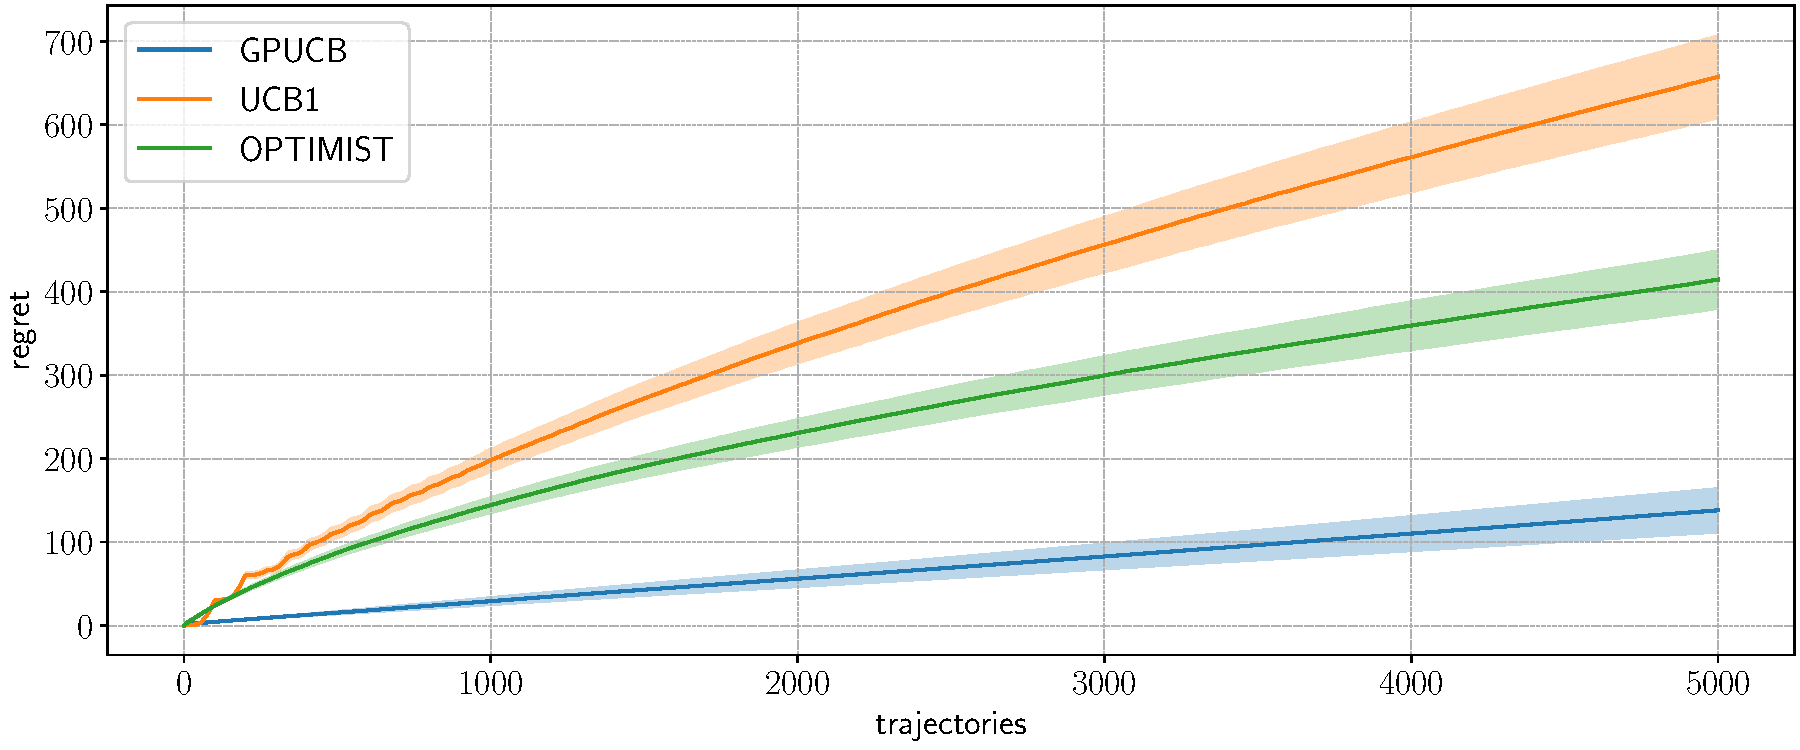
\includegraphics[width=\textwidth,height=\textheight,keepaspectratio]{Images/LQGcomparison.pdf}
\caption{Cumulative regret in
the \gls{LQG} experiment, comparing
\gls{OPTIMIST}, \gls{UCB}1 and \gls{GPUCB} when learning the mean hyperparameter only.
(30 runs, 95\% c.i.)}
\label{fig:LQGcomparison}
\end{figure}

\begin{figure*}[t!] 
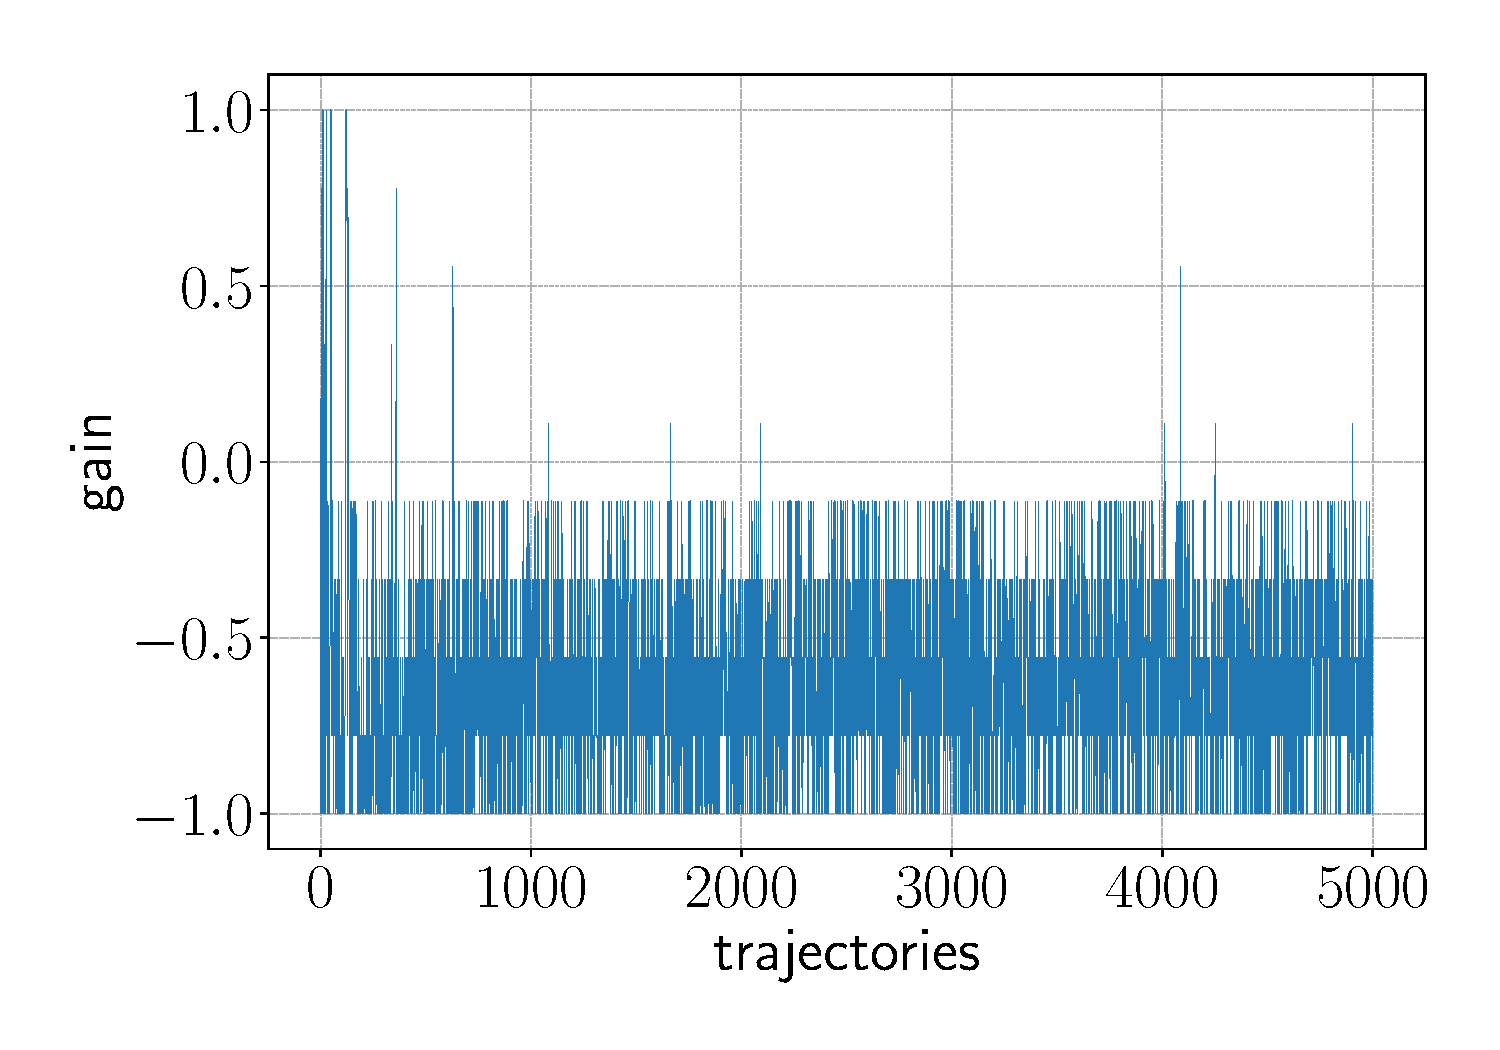
\includegraphics[width=.5\textwidth]{Images/LQG_GPUCB_mu.pdf}\hfill
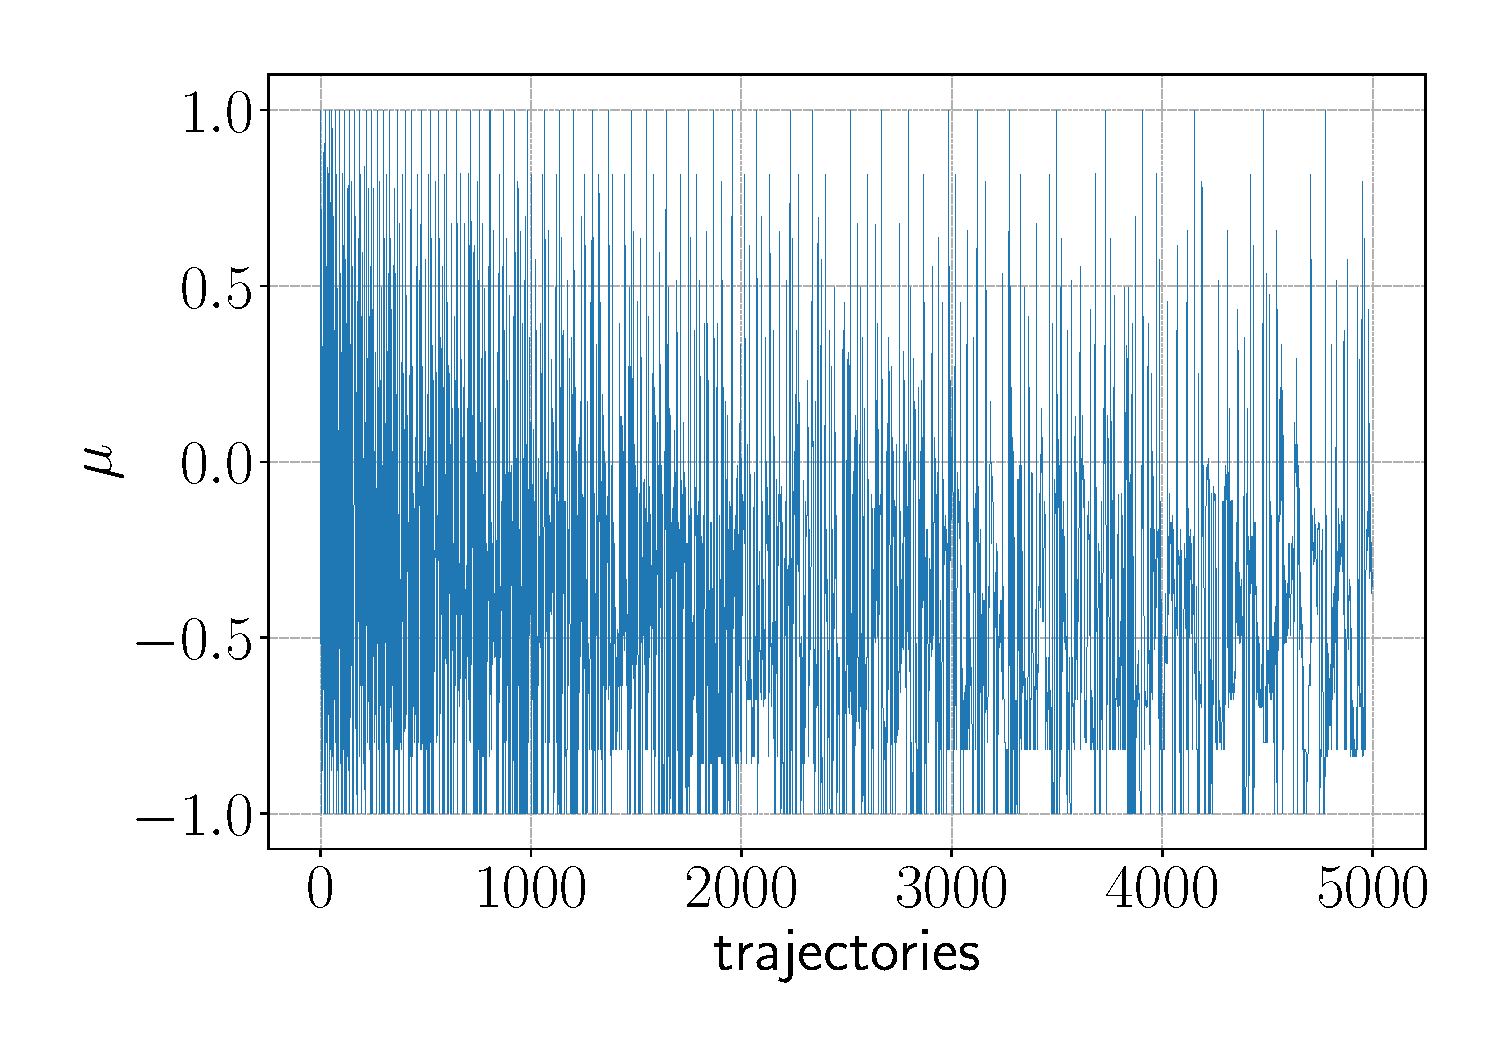
\includegraphics[width=.5\textwidth]{Images/LQG_OPTIMIST_mu.pdf}\hfill
%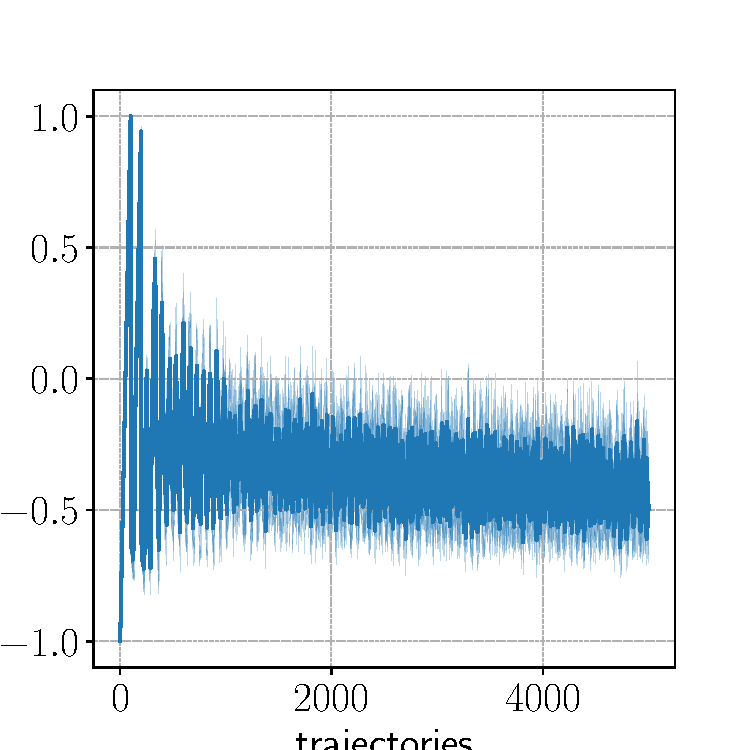
\includegraphics[width=.33\textwidth]{Images/LQG_UCB1_mu.pdf}
\caption{The gain parameter $\mu$ selected at each iteration of \gls{GPUCB}(left) and \gls{OPTIMIST}(right).}
\label{fig:LQGmu}
\end{figure*}


\begin{figure}[t!]
\centering
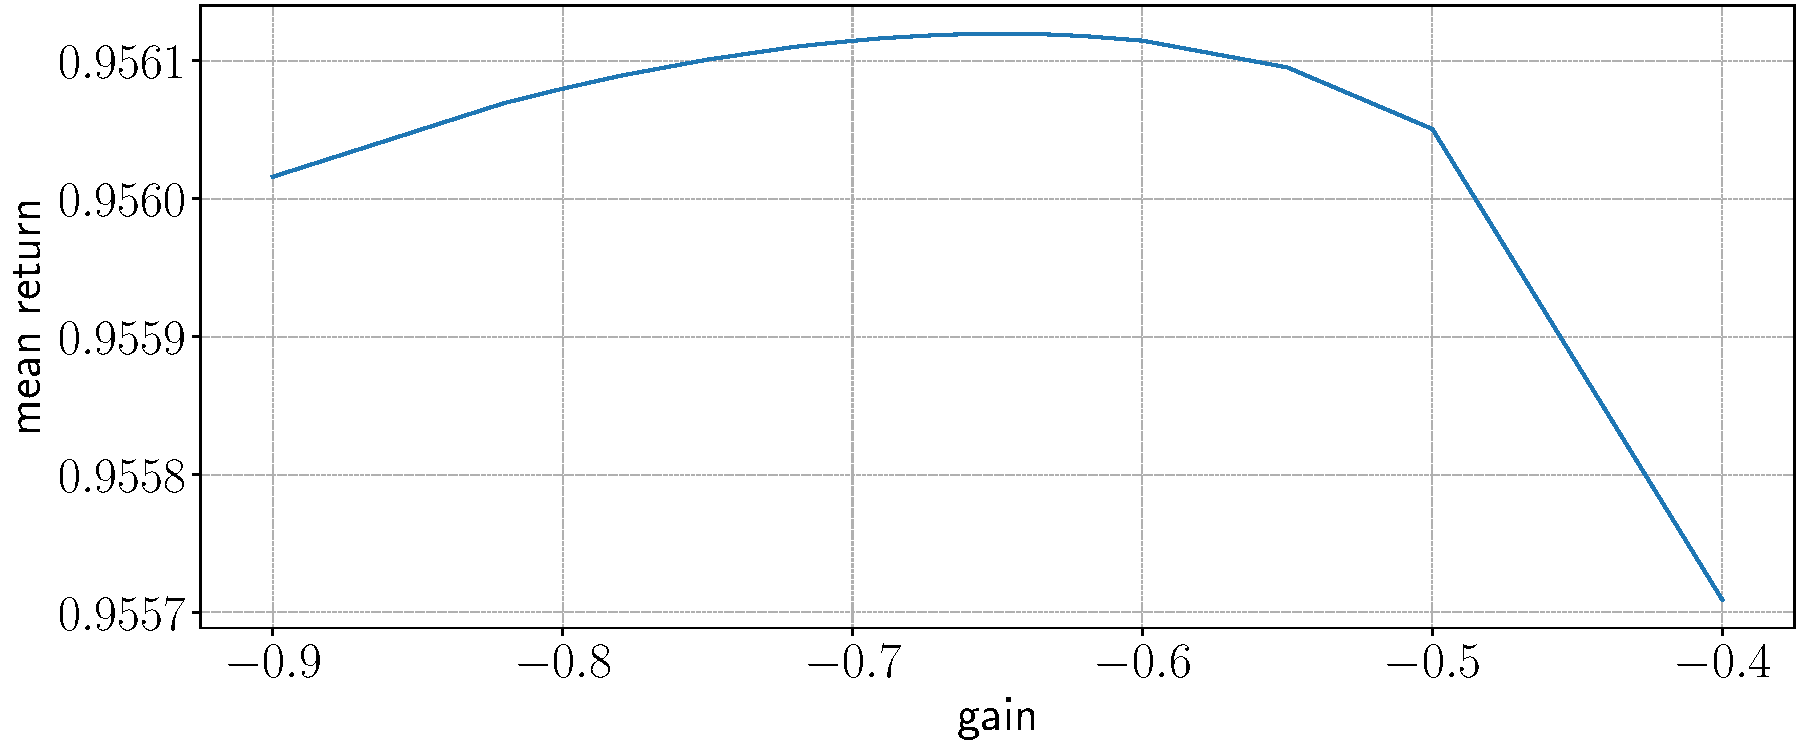
\includegraphics[width=.75\textwidth,keepaspectratio]{Images/LQG_optimal_gain.pdf}
\caption{Mean return of arms $\mu\in[-0.9,-0,5]$, calculated by averaging the return collected over 2000 trajectories for each arm pulled.}
\label{fig:LQGoptimalgain}
\end{figure}

In order to benchmark \gls{OPTIMIST} with both \gls{UCB}1 and \gls{GPUCB} on a discrete set, we first consider the case in which the only learnable parameter of $\nu_{\vxi}$ is the gain $\mu$. To this end, we consider a uniform discretization of the interval $[-1,1]$ made of 100 arms (every arm is a possible choice of $\mu$). The hyperpolicy standard deviation is fixed to $\sigma=0.1$. We experimented with different values of $\sigma$ and this turned out to be a good choice for making the task noisy enough, but not too noisy for obtaining interpretable results.\todo{spiegare cosa succede se $\sigma$ è troppo piccola e i bracci non condividono informazione} In Figure~\ref{fig:LQGcomparison}, we show the cumulative regret of the three algorithms, averaged over 30 runs. We can see that our algorithm significantly outperforms \gls{UCB}1.
Indeed, \gls{OPTIMIST} is able to exploit the structure of arms, \ie hyperpolicies, by means of the \gls{MIS} estimation, whereas \gls{UCB}1 does not make any assumption on arm correlation. In other words, \gls{OPTIMIST} performs a more informed, \ie directed, exploration, leveraging what the agent has experienced in past episodes more effectively. On the contrary, \gls{GPUCB} shows a better performance \wrt to \gls{OPTIMIST}. We point out that \gls{GPUCB} requires to specify, at the beginning of learning, the kernel of the Gaussian process from which the payoff function is sampled. We employed the default scikit-learn\footnote{A popular library for data mining and data analysis. Available at: https://scikit-learn.org/stable/} kernel, \ie the radial basis function kernel of the form:

\begin{align}
	k_T(\vx,\vx') &= \exp\left(-\lambda\norm{\vx-\vx'}^2\right),
\end{align}

where $\lambda$ is a free parameter. However, as it often happens in control tasks, our payoff is not actually sampled from a Gaussian process. This invalidates all theoretical guarantees of \gls{GPUCB} and may be at the root of the significantly more exploitative behavior \wrt \gls{UCB}1 and \gls{OPTIMIST} in the experiment. We can visualize the amount of exploration carried out by the three algorithms by looking at Figure (\ref{fig:LQGmu}), which depicts, at every iteration, the arm $\mu$ pulled by \gls{GPUCB} and \gls{OPTIMIST}. Indeed, \gls{OPTIMIST}explores the set of arms around the optimum much more extensively then \gls{GPUCB}, which, in the very first steps, commits to one arm near the optimum and never tries other arms again, if not for the noise induced by the positive variance $\sigma^2$ of the hyperpolicy. This is why \gls{GPUCB} regret is lower. In fact, in this setting the \gls{LQG} problem present a pretty wide set of optimal or near-optimal arms spanning in $[-0.9,-0.5]$, as shown in Figure (\ref{fig:LQGoptimalgain}).


\subsection{Gain and standard deviation}
In the second experiment on \gls{LQG}, we learn both the mean and the variance parameter of the Gaussian hyperpolicy: $\nu_{\vxi} = \mathcal{N}(\mu, \exp(2\sigma))$, where $\vxi=(\mu,\sigma)^T$ and we modeled with $\xi_2$ the standard deviation. The experiment coefficients are the same used before, shown in Table (\ref{tab:LQGcoeff}).
In Figure (\ref{fig:LQGcomparisonVar}), we show the cumulative regret averaged over 5 runs comparing \gls{OPTIMIST}, \gls{UCB}1 and \gls{GPUCB}. We see a trend similar to the case in which we learn only the mean parameter. While \gls{OPTIMIST} is able to exploit the structure of the arms induced by the fact that hyperpolicyes share information, beating \gls{UCB}1, \gls{GPUCB} still displays a better performance. The wider confidence intervals are a direct consequence of the wider spectrum of variances adopted by the hyperpolicy, bringing to very different policy parameters and, subsequently, very difference performance from one run to another.

\begin{figure*}[t!] 
\centering
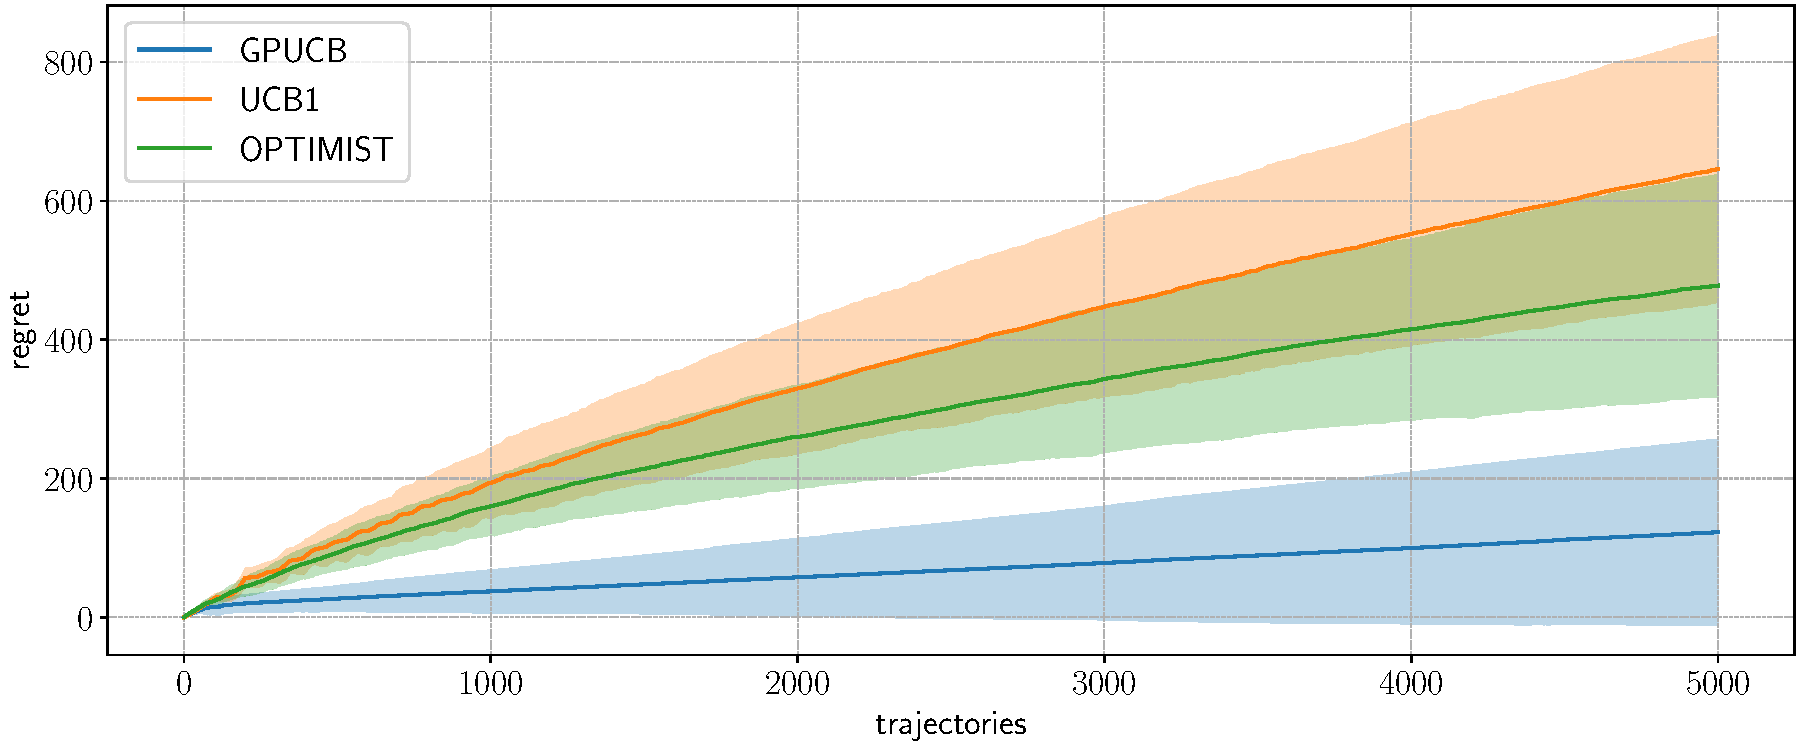
\includegraphics[width=\textwidth,height=\textheight,keepaspectratio]{Images/LQGcomparisonVar.pdf}
\caption{Cumulative regret in
the \gls{LQG} experiment, comparing
\gls{OPTIMIST}, \gls{UCB}1 and \gls{GPUCB} when learning both the mean and the standard deviation hyperparameters only.
(30 runs, 95\% c.i.)} 
\label{fig:LQGcomparisonVar} 
\end{figure*}

%%%%%%%%%%%%%%%%%%%%%%%%%%%%%%%%%%%%%%%%%%%%%%%%%%%%%%%%%%%%%%%%%%%%%%%%%%%%%%%%%%%%%%%%%%%%%%%%%%%%%%%%%%%%%%%%%%%%%%%%%%%%%%%%%%%

\section{Continuous Mountain Car}

\begin{figure*}[t!] 
\centering
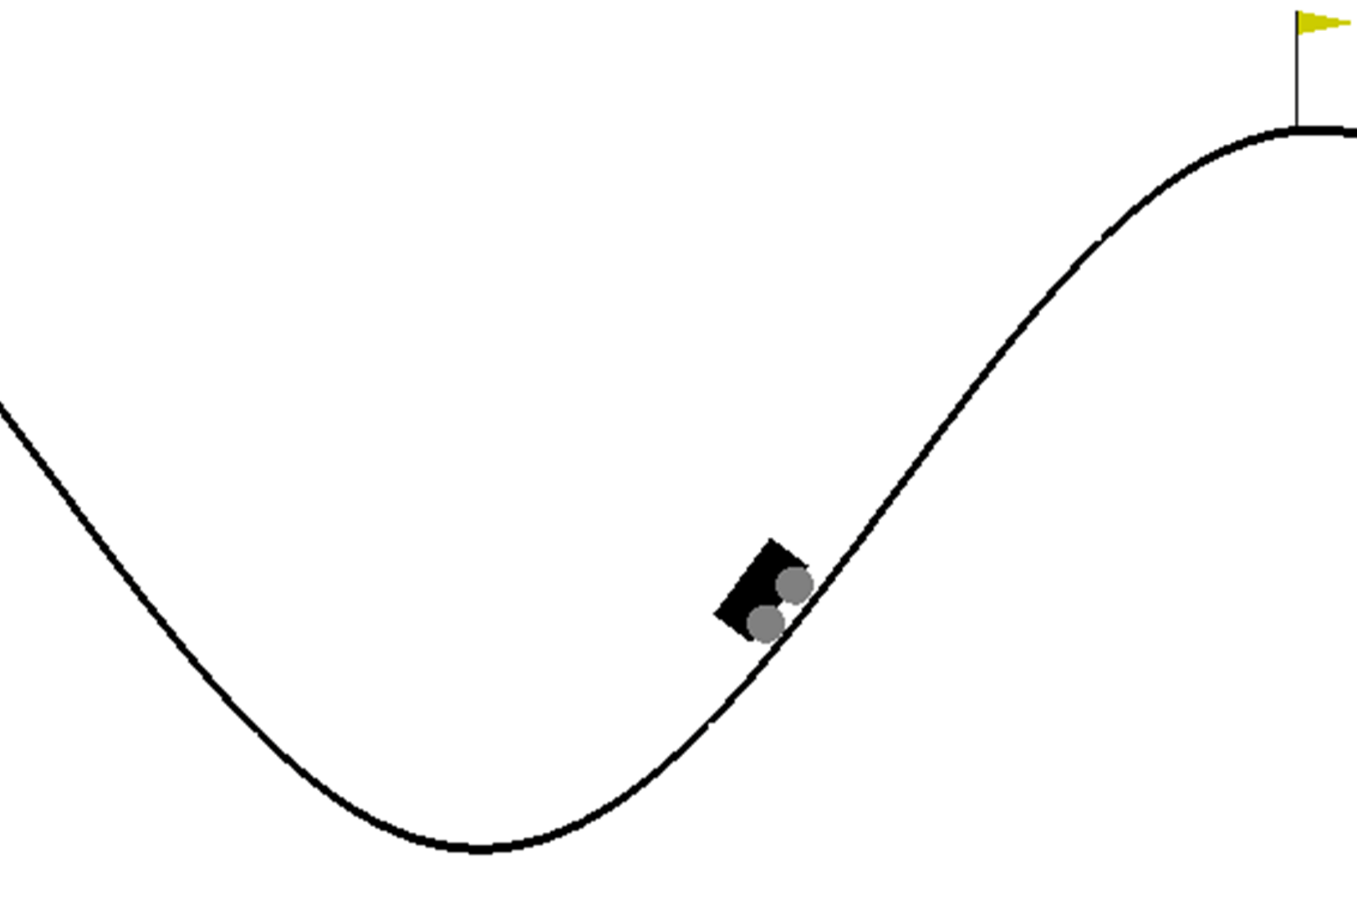
\includegraphics[width=.6\textwidth,keepaspectratio]{Images/MC.png}
\caption{Graphical representation of the Mountain Car problem.} 
\label{fig:MC}
\end{figure*} 

\begin{figure*}[t!] 
\centering
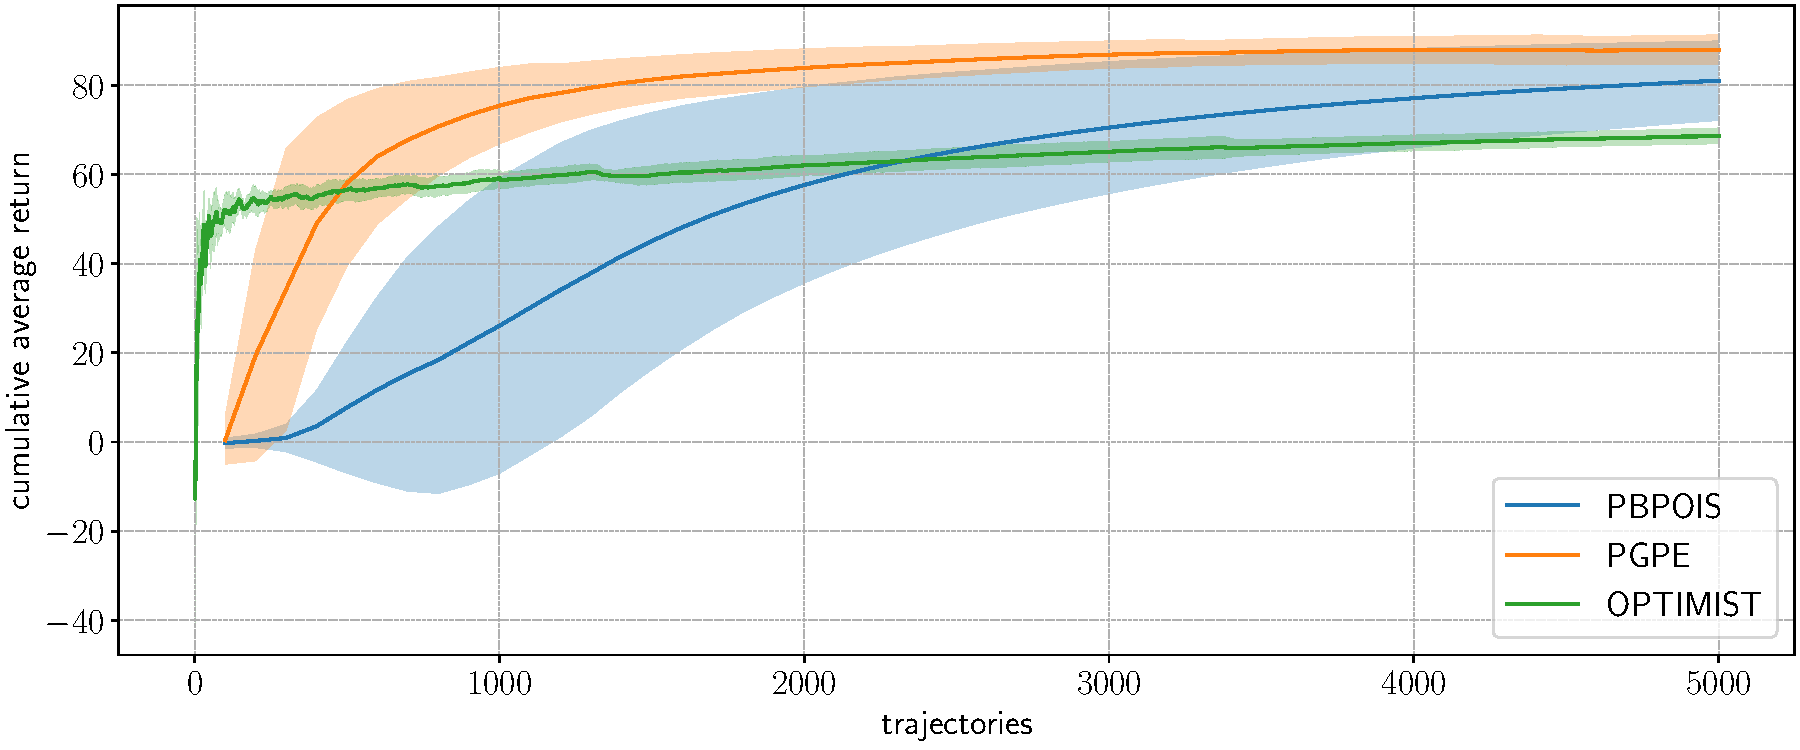
\includegraphics[width=\textwidth,height=\textheight,keepaspectratio]{Images/MC_mu.pdf}
\caption{Cumulative regret in
the \gls{LQG} experiment, comparing
\gls{OPTIMIST}, \gls{UCB}1 and \gls{GPUCB} when learning both the mean and the standard deviation hyperparameters only.
(30 runs, 95\% c.i.)} 
\label{fig:MCcomparison} 
\end{figure*}

The second experiment, illustrates the behaviour of \gls{OPTIMIST}2  
when the parameters of the hyperpolicy belong to a compact (continuous) space, on the continuous Mountain Car task\cite{brockman2016openai}. We chose the continuous Mountain Car because it is a simple, well known, continuous problem and has a sparse reward, which requires more exploration \wrt other simple challenges s.a. \gls{LQG}. 

In this problem, graphically represented in Figure (\ref{fig:MC}), the agent has to control the engine of an under-powered car in order to reach a target. The target is on top of a hill on the right-hand side of the car. If the car reaches it or goes beyond, the episode terminates. On the left-hand side, there is another hill. Climbing this hill can be used to gain potential energy and accelerate towards the target. On top of this second hill, the car cannot go further than a position equal to -1, as if there was a wall. The state space $\Sspace=[-1.2,0.6]x[-0.07,0.07]$ is constituted by a bi-dimensional vector with current position and velocity of the car. The action space $\Aspace\in\Reals$ is continuous: positive values correspond to a forward engine traction, negative values to backward engine traction. Every episode starts with the cat in a position between $-0.6$ and $-0.4$, with null velocity. 


In our experiment we use a Gaussian hyperpolicy with a two-dimensional learnable mean within a box $\vmu\in[-1,-1]\times[0,20]$ and a fixed covariance $\Cov=\mathrm{diag}(0.15,3)$. We compare \gls{OPTIMIST}2 (\ref{alg:2}) against parameter based policy optimization algorithms \gls{PGPE} (\ref{alg:PGPE}) and \gls{PBPOIS} \cite{metelli2018policy}. The latter is a parameter-based off-policy policy search algorithm which optimizes a lower bound of the performance estimator, built using single importance sampling. We chose to compare \gls{OPTIMIST} with \gls{PBPOIS} because of both their similarities and differences. In fact, despite being both off-policy algorithms based on importance sampling, \gls{PBPOIS} optimizes a lower bound on the performance, which implies a very limited exploration. By contrast, \gls{OPTIMIST} optimizes an upper bound on performance, accordingly to \gls{OFU} principle. Both algorithms are compared to \gls{PGPE}, that laid the foundations for both and is also known to lack proper exploration. 
The best learning rate $\alpha$ for \gls{PGPE} was searched in the set $[3, 2, 1, 0.1, 0.01, 0.001]$. For \gls{PBPOIS}, we used the suggested hyperparameters. \\

Results are shown in Figure (\ref{fig:MC}). We can notice that \gls{OPTIMIST}2 is able to learn a good policy in a very short time thanks to its better exploration capabilities. However, the policy gradient methods outperform it on the long run. In fact, the exploitative behaviour of the other two algorithms make them more performant \wrt \gls{OPTIMIST}, which continue to explore even after having found suitable parameters in few iterations. Even though these results might not be satisfactory from a performance point of view, our primary goal was to develop a \gls{PS} algorithm that would explore effectively the space of parameters. From this point of view, the results turn out to be successful. To convince ourselves of this claim, we refer to Figure (\ref{fig:MCgain}), in which we show the result of the kernel density estimation \cite{scott2015multivariate} of the probability of the two-dimensional learnable mean $\vmu$, for \gls{PGPE} (left) and \gls{OPTIMIST} (right). The estimation has been carried out by means of the Gaussian kernel density estimation available in the SciPy library.\footnote{https://docs.scipy.org/doc/} Intuitively, this represents the likelihood of each two-dimensional mean arm to be pulled by either \gls{PGPE} or \gls{OPTIMIST}. 

\begin{figure*}[t!] 
\centering
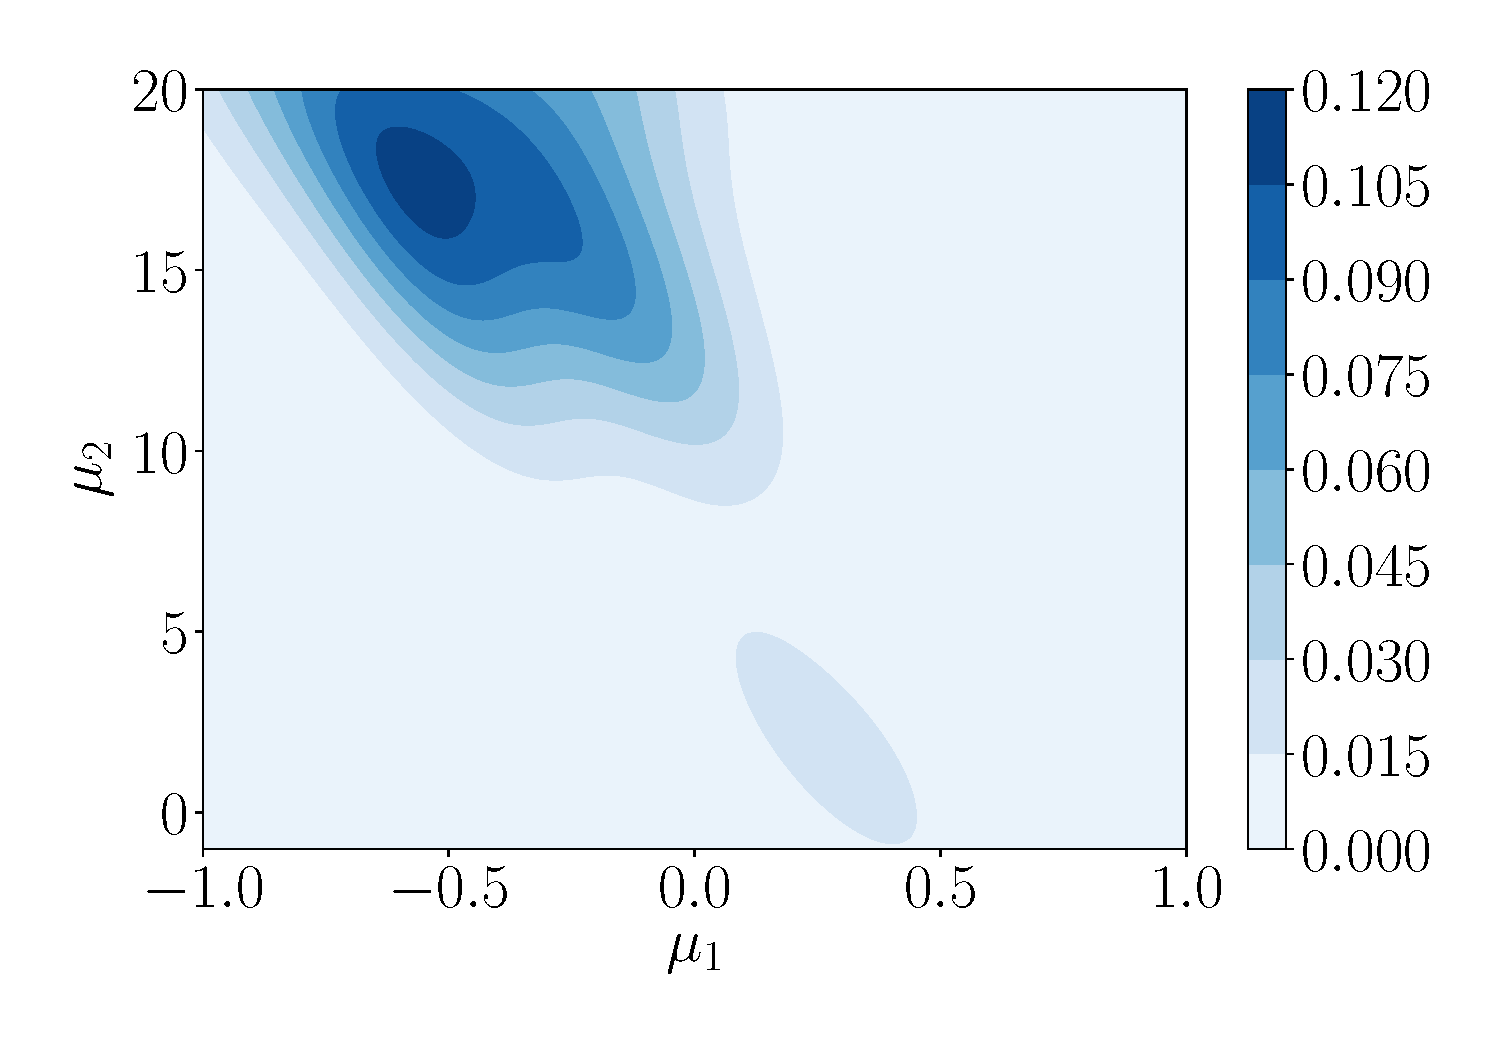
\includegraphics[width=.5\textwidth]{Images/MCgainPGPE.pdf}\hfill
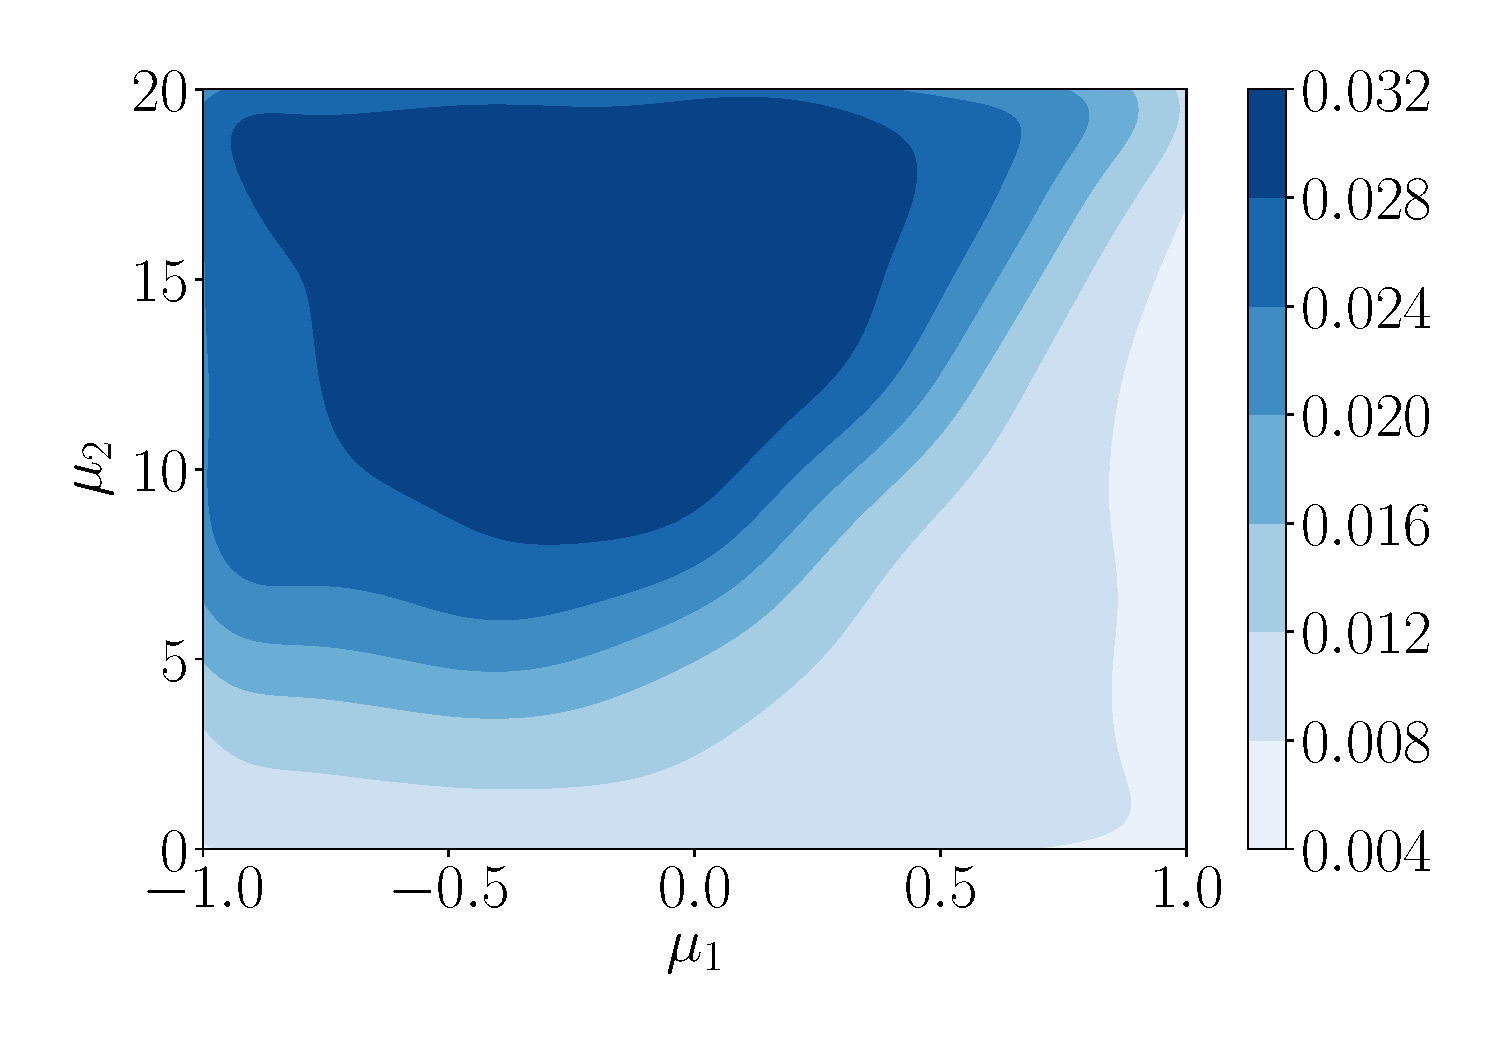
\includegraphics[width=.5\textwidth]{Images/MCgainOPTIMIST.pdf}
\caption{Gaussian kernel density estimation \cite{scott2015multivariate} of the probability of the two-dimensional learnable mean $\vmu$ to be pulled by either \gls{PGPE} (left) or \gls{OPTIMIST} (right).} 
\label{fig:MCgain}
\end{figure*} 